The protein structure is represented as the density maps of eleven atom types. 
We used the types shown in the Table \ref{Tbl:atomTypes}. Initially 21 atom types were proposed by X.Zou et al. 
\cite{huang2006iterative, huang2008iterative} using SYBYL rule set \cite{wang2006automatic}. In this work we clustered similar
types due to the hardware constraints. The density of an atom was modeled using the function: 
$$
\rho(r) =  \begin{cases}
               e^{-\frac{r^2}{2}}&r\leq 2.0\AA~\\
               0                 &r>2.0\AA~\\
            \end{cases}
$$
Each atom density was projected to the grid for the corresponding atom type. The resolution of the grid was set to 1\AA~ and the size of 
each grid to 120x120x120 cells.

\begin{table}[H]
\begin{center}
\begin{tabular}{ c | l | l }
    
    Type & Description & Atoms \\
    \hline
    1 & Sulfur containing atoms & CYSSG, METSD, MSESE \\ \hline
    2 & Amide nitrogens & ASNND2, GLNNE2, backbone N \\ \hline
    3 & Aromatic nitrogens & HISND1, HISNE2, TRPNE1 \\ \hline
    4 & Guanidine nitrogens & ARGNH1, ARGNH2, ARGNE \\ \hline
    5 & Nitrogen with three hydrogens & LYSNZ \\ \hline
    6 & Carboxyl oxygen & ACEO, ASNOD1, GLNOE1, backbone O \\ \hline
    7 & Oxygen in hydroxyl group & SEROG, THROG1, TYROH \\ \hline
    8 & Oxygen in carboxyl group and terminus oxygen & ASPOD1, ASPOD2, GLUOE1, GLUOE2, \\
     & &  O-terminal, OT2-terminal, OXT-terminal \\ \hline
    9 & Sp2 carbon & ARGCZ, ASPCG, GLUCD, ACEC, \\
     & & ASNCG, GLNCD, backbone C \\ \hline
    10 & Aromatic carbon & HISCD2, HISCE1, HISCG, PHECD1 \\
     & & PHECD2, PHECE1, PHECE2, PHECG \\ 
     & & PHECZ, TRPCD1, TRPCD2, TRPCE2 \\
     & & TRPCE3, TRPCG, TRPCH2, TRPCZ2 \\
     & & TRPCZ3, TYRCD1, TYRCD2, TYRCE1 \\
     & & TYRCE2, TYRCG, TYRCZ \\ \hline
    11 & Sp3 carbon & ALACB, ARGCB, ARGCG, ARGCD \\
     & & ASNCB, ASPCB, GLNCB, GLNCG \\
     & & GLUCB, GLUCG, HISCB, HISCB \\
     & & ILECB, ILECD1, ILECG1, ILECG2 \\
     & & LEUCB, LEUCD1, LEUCD2, LEUCG \\
     & & LYSCB, LYSCD, LYSCG, LYSCE \\
     & & METCB, METCE, METCG, MSECB \\
     & & MSECE, MSECG, PHECB, PROCB \\
     & & PROCG, PROCD, SERCB, THRCG2 \\
     & & TRPCB, TYRCB, VALCB, VALCG1 \\
     & & VALCG2, ACECH3, THRCB, CYSCB \\
     & & backbone CA \\ \hline
    
\end{tabular}
    
    \caption {Atom types used in this work. In the atom notation the first three letters are the name of an aminoacid and the rest is 
    the atom name in the PDB format.}
    \label{Tbl:atomTypes}
\end{center}
\end{table}
Figure \ref{Fig:atomic_densities} shows an example of atomic densities of a peptide with the PDB code 5eh6.
Only non-zero densities are shown.

\begin{figure}[H]
    \centering
    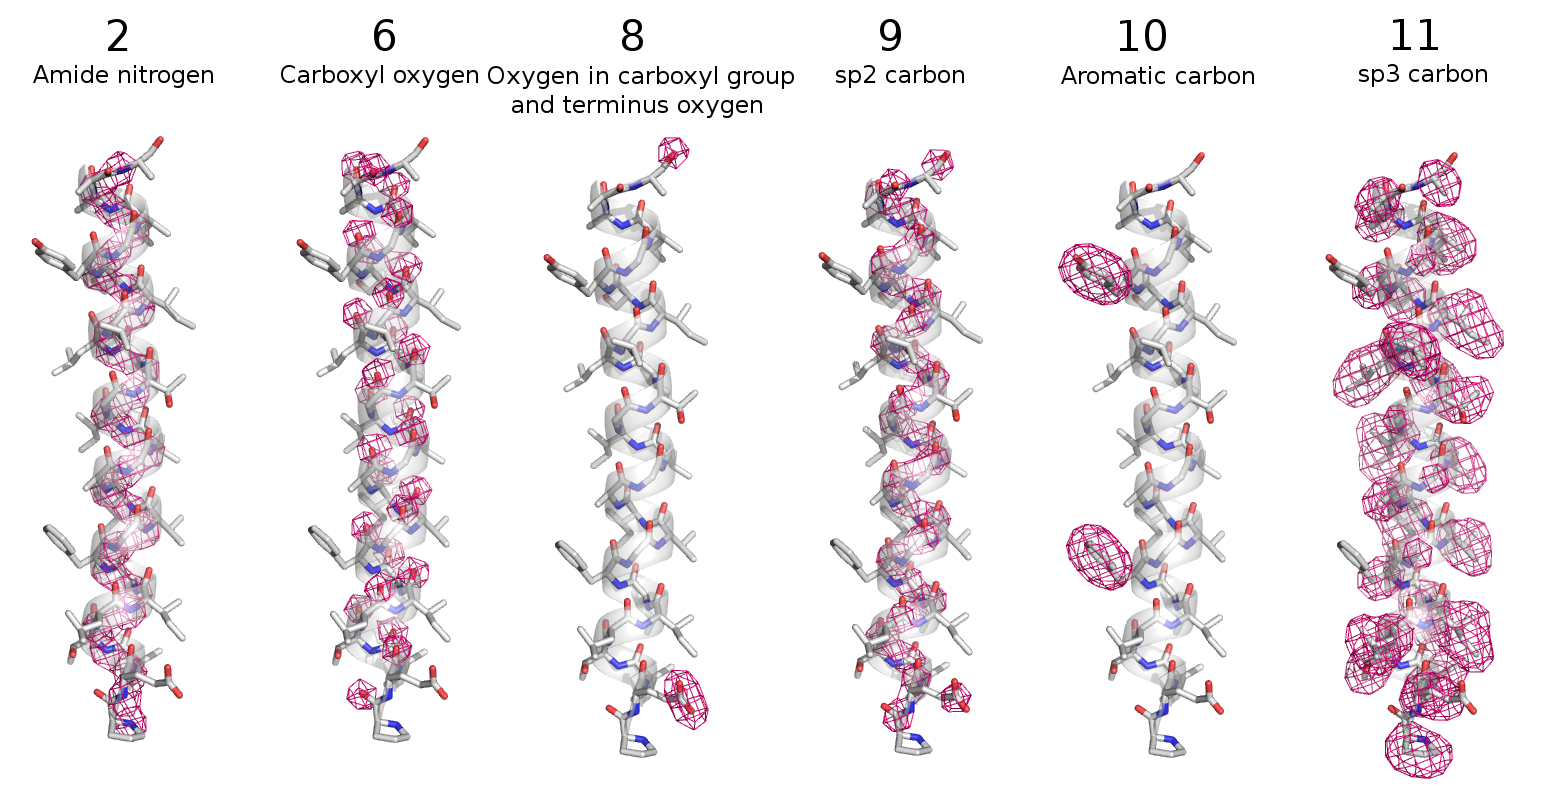
\includegraphics[width=\linewidth]{Fig/atomic_densities_V3.png}
    \caption{The example of the representation of a protein using atomic densities. The density map is 
    shown using the volumetric rendering plugin for PyMol. The pdb-code of the protein used for this visualization is 5eh6.
    The isosurface level was set to $0.5$.}
    \label{Fig:atomic_densities}
\end{figure}